%% Exemplo de utilizacao do estilo de formatacao normas-utf-tex (http://normas-utf-tex.sourceforge.net)
%% Autores: Hugo Vieira Neto (hvieir@utfpr.edu.br)
%%          Diogo Rosa Kuiaski (diogo.kuiaski@gmail.com)
%% Colaboradores:
%%          C?zar M. Vargas Benitez <cesarvargasb@gmail.com>
%%          Marcos Talau <talau@users.sourceforge.net>


\documentclass[openright]{normas-utf-tex} %openright = o capitulo comeca sempre em paginas impares
%\documentclass[oneside]{normas-utf-tex} %oneside = para dissertacoes com numero de paginas menor que 100 (apenas frente da folha) 


\usepackage[alf,abnt-emphasize=bf,bibjustif,recuo=0cm, abnt-etal-cite=2, abnt-etal-list=99]{abntcite} %configuracao correta das referencias bibliograficas.

\usepackage[utf8]{inputenc}

\usepackage{float}% deixar tabelas no lugar

\usepackage{booktabs} %para gerar tabelas

\usepackage[brazil]{babel} % pacote portugues brasileiro

\usepackage[T1]{fontenc}

\usepackage{amsmath,amsfonts,amssymb} % pacote matematico
\usepackage{graphicx} % pacote grafico
\usepackage{times} % fonte times

%Podem utilizar GEOMETRY{...} para realizar pequenos ajustes das margens. Onde, left=esquerda, right=direita, top=superior, bottom=inferior. P.ex.:
%\geometry{left=3.0cm,right=1.5cm,top=4cm,bottom=1cm} 

% ---------- Preambulo ----------
\instituicao{Universidade Tecnol\'ogica Federal do Paran\'a} % nome da instituicao
\programa{} % nome do programa
\area{Engenharia de Computação} % [Engenharia Biom\'edica] ou [Inform\'atica Industrial] ou [Telem\'atica]

\documento{Relatório} % [Disserta\c{c}\~ao] ou [Tese]
\nivel{Graduação} % [Mestrado] ou [Doutorado]
\titulacao{Graduação} % [Mestre] ou [Doutor]

\titulo{\MakeUppercase{Projeto 2}}

\autor{Aline Kolczycki Borges}
\autordois{Guilherme Jacichen}
\autortres{Jessica Isoton Sampaio}% autor do trabalho

\comentario{Relatório de atividade prática apresentado à disciplina de Entrônica 2, do departamento de Eletrônica como requisito parcial do curso de Engenharia de Computação da UTFPR.}

\local{Curitiba} % cidade
\data{\the\year} % ano automatico


%---------- Inicio do Documento ----------
\begin{document}

\capa % geracao automatica da capa
\folhaderosto % geracao automatica da folha de rosto
%\termodeaprovacao % <- ainda a ser implementado corretamente

% sumario
\sumario % geracao automatica do sumario
\listoffigures
\listoftables

%---------- Inicio do Texto ----------
% recomenda-se a escrita de cada capitulo em um arquivo texto separado (exemplo: intro.tex, fund.tex, exper.tex, concl.tex, etc.) e a posterior inclusao dos mesmos no mestre do documento utilizando o comando \input{}, da seguinte forma:
%\input{intro.tex}
%\input{fund.tex}
%\input{exper.tex}
%\input{concl.tex}


%---------- Primeiro Capitulo ----------
\chapter{Introdução}
\label{intro}

Amplificadores convencionais sem realimentação possuem alguns inconvenientes: são difíceis de se controlar o ganho, não possuem muita flexibilidade para alterar sua amplificação, possuem muitas vezes uma banda estreita, a degradação dos elementos semicondutores altera muito suas propriedades e podem apresentar carácterísticas como impedância de entrada e de saída fora do desejado. À estes circuitos chamamos de amplificador de malha aberta devido à sua representação como um diagrama de bloco (figura \ref{fig:blocos_malha_aberta}). \cite{pedroni,millman} 

Circuitos amplificadores realimentados melhoram à estabilidade do ganho, mantendo-o mais independente de fatores externos, melhoram a qualidade das impedâncias de entrada e saída, diminuem as distorções dos sinais, aumentam a banda de resposta e são flexíveis para o controle do ganho. Entretanto, algumas desvantagens também são encontradas como dissipação de potência extra devido ao efeito de carga e a amplificação menor. Estes circuito também são conhecidos como amplificadores de malha fechada por sua representação no diagrama de blocos (figura \ref{fig:blocos_malha_fechada}). \cite{pedroni,millman} 

\begin{figure}[H]
\centering
\begin{minipage}{0.45\textwidth}
\centering
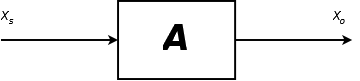
\includegraphics[width=1.0\linewidth]{img/BlocosMalhaAberta.png}
\caption{Representação de um sistema (amplificador) malha aberta.}
Fonte: Autoria própria
\label{fig:blocos_malha_aberta}
\end{minipage}\hfill
\begin{minipage}{0.45\textwidth}
\centering
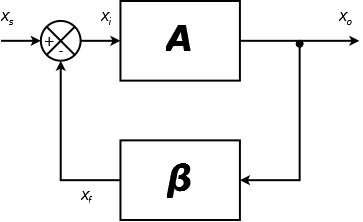
\includegraphics[width=1.0\linewidth]{img/BlocosMalhaFechada.png}
\caption{Representação de um sistema (amplificador realimentado) malha fechada.}
Fonte: Autoria própria
\label{fig:blocos_malha_fechada}
\end{minipage}
\end{figure}

\section{Revisão Bibliográfica}
\label{rev_bib}

De acordo com a imagem \ref{fig:blocos_malha_fechada}, tira-se as equações \ref{eq:X_i_X_s_X_f}, \ref{eq:X_o_A_X_i}, \ref{eq:X_f_beta_X_o}, e através delas é possível fazer a dedução da equação \ref{eq:ganho_malha_fechada_genérico}, que seria o ganho em malha fechada do amplifcador em função da realimentação $\beta$ e do ganho do amplifcador de malha aberta $A$.\cite{pedroni,millman} 

\begin{equation} \label{eq:X_i_X_s_X_f}
X_i = X_s - X_f
\end{equation}

\begin{equation} \label{eq:X_o_A_X_i}
X_o = A \cdot X_i 
\end{equation}

\begin{equation} \label{eq:X_f_beta_X_o}
X_f = \beta \cdot X_o
\end{equation}

\begin{equation}\label{eq:ganho_malha_fechada_genérico}
A_f = \frac{X_o}{X_s} = \frac{X_o}{X_i + X_f} = \frac{1}{\frac{X_i}{X_o}+\frac{X_f}{X_o}} = \frac{1}{\frac{1}{A}+\beta} = \frac{A}{1+\beta \cdot A}
\end{equation}

O fator de dessensibilidade $D$ do amplificador realimentado é definido como o inverso sensibilidade completa do amplificador de malha fechada de acordo com a equação \ref{eq:dessensibilidade}. A sensibilidade simples do amplificador é dada pela equação \ref{eq:sensibilidade_simples}, e a partir dela pode ser deduzido a sensibilidade completa da equação \ref{eq:sensibilidade_completa}. Substituindo a equação \ref{eq:dessensibilidade} em \ref{eq:ganho_malha_fechada_genérico}  obtemos a equação \ref{eq:ganho_dessensibilidade}. \cite{pedroni,millman} 

\begin{equation} \label{eq:sensibilidade_simples}
Ss^{A_f}_{A} = \displaystyle \frac{dA_f}{dA} = \frac{\left(1+\beta \cdot A\right) - \beta \cdot A}{\left(1 + \beta \cdot A\right)^2} = \frac{1}{\left(1 + \beta \cdot A \right)^2}
\end{equation}

\begin{equation} \label{eq:sensibilidade_completa}
S^{A_f}_{A} = Ss^{A_f}_{A} \cdot \frac{A_Q}{A_{fQ}} = \frac{1}{\left(1 + \beta \cdot A \right)^2} \cdot \frac{A}{\frac{A}{1+\beta \cdot A}} = \frac{1}{\left(1 + \beta \cdot A \right)}
\end{equation}

\begin{equation} \label{eq:dessensibilidade}
D = \left(S^{A_f}_{A}\right)^{-1} =1 + \beta \cdot A
\end{equation}

\begin{equation}\label{eq:ganho_dessensibilidade}
A_f = \frac{A}{D} 
\end{equation}

\subsection{Topologia série de tensão}

Um circuito de realimentação do tipo série de tensão (ou tensão série, ou malha-nó, ou série-paralelo) possui a representação da figura \ref{fig:serie_tensao}. Nela, o parâmetro comum ao amplificador e a realimentação é a corrente de entrada $I_i$ e o parâmetro amostrado é a tensão de saída $V_o$. \cite{millman,pedroni}

\begin{figure}[ht]
\centering
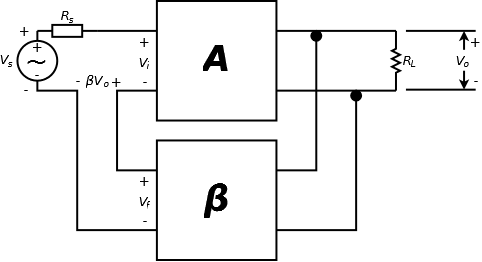
\includegraphics[width=0.75\linewidth]{img/SerieTensao.png}
\caption{Representação de uma realimentação série de tensão}
Fonte: Autoria própria
\label{fig:serie_tensao}
\end{figure}

A análise do circuito requer passagem para forma de quadripolos, de acordo com a figura \ref{fig:serie_tensao_quad}, onde foi utilizado o equivalente $h$.  \cite{millman,pedroni}

\begin{figure}[ht]
\centering
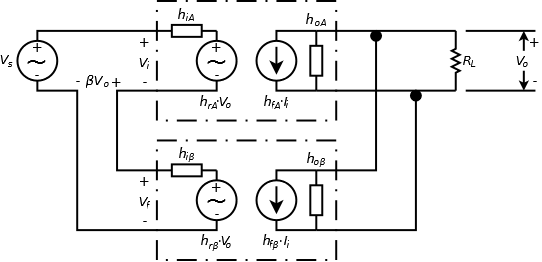
\includegraphics[width=0.75\linewidth]{img/SerieTensaoQuad.png}
\caption{Realimentação série de tensão com quadripolos na configuração $h$.}
Fonte: Autoria própria
\label{fig:serie_tensao_quad}
\end{figure}

Segundo \citeonline{millman}, são ainda aplicáveis três hipóteses que simplificam a análise deste circuito:

\begin{itemize}
\item O sinal de entrada é transmitidade apenas pelo amplificador, e não pela realimentação. Em outras palavras, $h_{f\beta} = 0$.
\item O sinal de realimentação é transmitido apenas pelo elo de realimentação, e não pelo amplificador. Em outras palavras, $h_{rA} = 0$.
\item O fator de realimentação $\beta$ não depende das resistências de carga $R_L$ e da resistência da fonte de sinal $R_S$.
\end{itemize}
Considerando estas hipóteses simplificadoras, o circuito obtido será representado pela figura \ref{fig:serie_tensao_quad_simp}. 

\begin{figure}[ht]
\centering
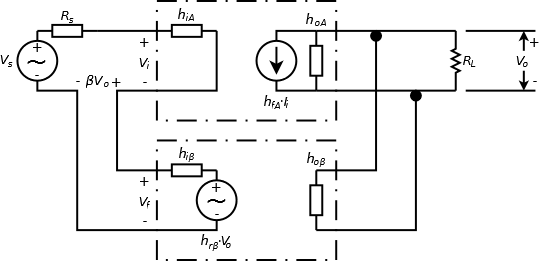
\includegraphics[width=0.75\linewidth]{img/SerieTensaoQuadSimp.png}
\caption{Realimentação série de tensão aplicando-se as hipóteses simplificadoras.}
Fonte: Autoria própria
\label{fig:serie_tensao_quad_simp}
\end{figure}

Como pode ser percebido, o fato de incluirmos um circuito a mais ao amplificador altera seu comportamento devido à impedâncias adicionais que entram no circuito (figura \ref{fig:serie_tensao_efeito_carga}). Assim, os calculos envolvendo o amplificador realimentado devem considerar que seu equivalente sem realimentação possui este efeito de carga. \cite{pedroni,millman}

\begin{figure}[H]
\centering
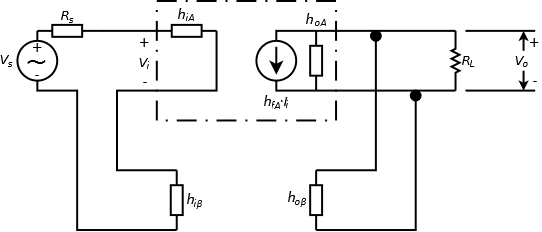
\includegraphics[width=0.75\linewidth]{img/SerieTensaoEfeitoCarga.png}
\caption{Efeito de carga sobre um circuito com realimentação série de tensão.}
Fonte: Autoria própria
\label{fig:serie_tensao_efeito_carga}
\end{figure}

A partir da figura \ref{fig:serie_tensao_quad}, tiramos as equações de nós e malhas em \ref{eq:ded_par_tensao}. Agrupando os termos em evidência, manipulando-os e considerando $G_L = \frac{1}{R_L}$ tem-se o sistema \ref{eq:ded_pt_evid}.

\begin{equation}\label{eq:ded_par_tensao}
\begin{cases}
V_s + h_{rA} \cdot V_o + h_{r\beta} \cdot V_o = R_s \cdot I_i + h_{iA} \cdot I_i + h_{i\beta} \cdot I_i

\\
h_{fA} \cdot I_i + h_{f\beta} \cdot I_i = \frac{V_o}{R_L} + h_{oA} \cdot V_o + h_{o\beta} \cdot V_o
\end{cases}
\end{equation}

\begin{equation}\label{eq:ded_pt_evid}
\begin{cases}
\frac{V_s}{V_o} = \frac{I_i}{V_o} \cdot \left( R_s + h_{iA} + h_{i\beta} \right) - \left( h_{rA} + h_{r\beta} \right)

\\
\frac{I_i}{V_o} =  \frac{\left( G_L + h_{oA} + h_{o\beta} \right)}{\left( h_{fA} + h_{f\beta} \right)}
\end{cases}
\end{equation}

A partir do sistema \ref{eq:ded_pt_evid} obtém-se \ref{eq:ded_pt_2} se for substituido o segundo termo no primeiro (onde as relações \ref{eq:st_imp_ent_quad} e \ref{eq:st_imp_saida_quad} são utilizadas) e invertendo o resultado.

\begin{equation}\label{eq:ded_pt_2}
\frac{V_s}{V_o} = \frac{Z_i \cdot Y_o}{\left( h_{fA} + h_{f\beta} \right)} - \left( h_{rA} + h_{r\beta}\right)
\end{equation}

\begin{equation}\label{eq:st_imp_ent_quad}
Z_i = h_{iA} + h_{i\beta} + R_s
\end{equation}

\begin{equation}\label{eq:st_imp_saida_quad}
Y_o = h_{oA} + h_{o\beta} + G_L
= h_{oA} + h_{o\beta} + \frac{1}{R_L}
\end{equation}

Manipulando a equação \ref{eq:ded_pt_2}, chega-se em \ref{eq:ded_pt_fb}, que possui muita semelhança com a equação \ref{eq:ganho_malha_fechada_genérico}, onde as relações \ref{eq:st_amp_quad} e \ref{eq:st_beta_quad} podem ser aplicadas para a equação ficar identica. Como se pode perceber em \ref{eq:st_amp_quad}, o ganho realimentado depende do efeito de carga ($Z_i$ e $Y_o$), e quando consideradas as hipóteses simplificadoras, apenas o ganho do amplificador de malha aberta aparece em $A_{Vs}$ aparece (o mesmo vale para $\beta$). \cite{pedroni,millman}

\begin{equation}\label{eq:ded_pt_fb}
A_{Vs_f} = \frac{V_o}{V_s} = \left(\frac{V_s}{V_o}\right)^{-1} =
\frac{-\frac{h_{fA} + h_{f\beta} } {Z_i \cdot Y_o}} { 1 + \left(h_{rA} + h_{r\beta}\right) \cdot \left(-\frac{h_{fA} + h_{f\beta}} {Z_i \cdot Y_o} \right)}
\end{equation}

\begin{equation}\label{eq:st_amp_quad}
A_{Vs} = -\frac{h_{fA} + h_{f\beta}} {Z_i \cdot Y_o}
\end{equation}

\begin{equation}\label{eq:st_beta_quad}
\beta = h_{rA} + h_{r\beta}
\end{equation}

\begin{equation}\label{eq:st_D}
D = 1 + \left(h_{rA} + h_{r\beta}\right) \cdot \left(-\frac{h_{fA} + h_{f\beta}} {Z_i \cdot Y_o} \right)
\end{equation}

Agora será calculado as impedâncias de entradas e saída. O sistema \ref{eq:ded_pt_imp_ent} provém do sistema \ref{eq:ded_pt_evid}, enquanto a equação \ref{eq:ded_pt_imp_ent2} é resultado da divisão do primeiro termo por $I_s$ e da substituição de $V_o$ pelo segundo termo do sistema mencionado primeiramente. Substituindo nesta equação os termo das equações \ref{eq:st_imp_ent_quad} e \ref{eq:st_imp_saida_quad} ($Z_i$ e $Y_o$) e deixando $Z_i$ em evidência, é possível obter a equação \ref{eq:st_imp_ent_fb} se substituirmos o termo equivalente à dessensibilidade dada em \ref{eq:st_D}. \cite{pedroni,millman}

\begin{equation}\label{eq:ded_pt_imp_ent}
\begin{cases}
V_s = I_i \cdot \left( R_s + h_{iA} + h_{i\beta} \right) - V_o \cdot \left( h_{rA} + h_{r\beta} \right)

\\
V_o =  I_i \cdot \frac{\left( h_{fA} + h_{f\beta} \right)}{\left( G_L + h_{oA} + h_{o\beta} \right)}
\end{cases}
\end{equation}

\begin{equation}\label{eq:ded_pt_imp_ent2}
\frac{V_s}{I_i} = \left( R_s + h_{iA} + h_{i\beta} \right) + \left(h_{rA} + h_{r\beta}\right) \cdot \left(-\frac{h_{fA} + h_{f\beta}} {\left( G_L + h_{oA} + h_{o\beta} \right)} \right)
\end{equation}

\begin{equation}\label{eq:st_imp_ent_fb}
Z_{i_f} = Z_i \cdot \left( 1 + \left(h_{rA} + h_{r\beta}\right) \cdot \left(-\frac{h_{fA} + h_{f\beta}} {Z_i \cdot Y_o} \right) \right) = Z_i \cdot D
\end{equation}

Para calcular a impedância de saída, temos que a corrente total na carga é dada pela equação \ref{eq:ded_pt_imp_saida}, enquanto a corrente de entrada é encontrada através da equação \ref{eq:ded_pt_imp_ent2}. Substituindo $I_i$ em \ref{eq:ded_pt_imp_saida} por \ref{eq:ded_pt_imp_saida2} obtém-se \ref{eq:ded_pt_imp_saida3}. Substituindo nesta equação os termo das equações \ref{eq:st_imp_ent_quad} e \ref{eq:st_imp_saida_quad} ($Z_i$ e $Y_o$) e deixando $Y_o$ em evidência, é possível obter a equação \ref{eq:st_imp_ent_fb} se substituirmos o termo equivalente à dessensibilidade dada em \ref{eq:st_D}. A impedância de saída será o oposto da condutância encontrada, ou seja, $Z_{o_f} = \frac{Z_o}{D}$. \cite{pedroni,millman}

\begin{equation}\label{eq:ded_pt_imp_saida}
I_{o} = I_i \cdot \left( h_{fA} + h_{f\beta} \right) + V_o \cdot \left(G_L + h_{oA} + h_{o\beta} \right)
\end{equation}

\begin{equation}\label{eq:ded_pt_imp_saida2}
I_{i} =  V_o \cdot \frac{\left(h_{rA} + h_{r\beta}\right)}{\left( R_s + h_{iA} + h_{i\beta} \right)}
\end{equation}

\begin{equation}\label{eq:ded_pt_imp_saida3}
\frac{I_o}{V_o} = \left( G_L + h_{oA} + h_{o\beta} \right) + \left(h_{rA} + h_{r\beta}\right) \cdot \left(-\frac{h_{fA} + h_{f\beta}} {\left( G_L + h_{oA} + h_{o\beta} \right)} \right)
\end{equation}

\begin{equation}\label{eq:st_imp_saida_fb}
Y_{o_f} = Y_o \cdot \left( 1 + \left(h_{rA} + h_{r\beta}\right) \cdot \left(-\frac{h_{fA} + h_{f\beta}} {Z_i \cdot Y_o} \right) \right) = Y_o \cdot D
\end{equation}

As duas impedâncias encontradas dependem de $R_L$ e $R_s$, que não são parâmetro próprios do amplificador. Para enontrar as impedâncias próprias do amplificador $Z'_i$ e $Z'_o$, deve-se aplicar os limites $R_s \rightarrow 0$ e $R_L \rightarrow \infty$. \cite{pedroni}

\subsection{Instabilidade}

Para resposta em frequência de circuitos realimentados, utiliza-se a equação \ref{eq:ganho_malha_fechada_genérico} como uma função onde os ganhos dependem da frequência, como na equação \ref{eq:ganho_malha_fechada_freq}.  \cite{pedroni,millman}


\begin{equation}\label{eq:ganho_malha_fechada_freq}
A(s)_f = \frac{A(s)}{1+\beta \cdot A(s)}
\end{equation}

A análise desta função revela algumas propriedades com relação ao produto $\beta \cdot A(s)$. Se $\beta \cdot A(s) > 0$ teremos uma realimentação negativa, e o circuito será estável. Se -1 < $\beta \cdot A(s) < 0$, então teremos uma realimentação positiva, e o sinal será regenerativo, isto é, ele continuará a existir mesmo que a entrada seja 0. \cite{pedroni,millman}

Nisto se constitui a instabilidade, sendo que o sinal negativo é determinado por $A(s)$. Caso haja um deslocamento de fase de 90-180º, o sinal do amplificador terá sentido inverso ao original. Com deslocamento de 180º, o modulo de $Av(s)$ é o mesmo, entretanto seu sinal será negativo. Portanto, para se evitar a instabilidade deve-se análisar a resposta em frequência da fase e garantir que o amplificador não irá inverter a fase no regime de trabalho. \cite{pedroni,millman}

Uma outra maneira de visualizar o problema é considerando o ganho $Av(s)$ como uma divisão de polinômios (equação \ref{eq:av_div_poli}), com um numerador ($N(s)$) e um denominador ($D(s)$). Esta consideração no ganho realimentado leva à equação \ref{eq:avf_div_poli}, que não possuirá os mesmos pólos da equação \ref{eq:av_div_poli}. A variação de $\beta$ neste caso irá deslocar os pólos pelo plano imaginário na função de transferência. Se algum pólo existir no semiplano positivo do \textit{root locus}, o circuito assumirá instabilidade. Não será demonstrado aqui, mas segundo \citeonline{millman}, circuitos com mais de 2 pólos sempre será instável.

\begin{equation}\label{eq:av_div_poli}
Av(s) = \frac{N(s)}{D(s)}
\end{equation}


\begin{equation}\label{eq:avf_div_poli}
Av(s)_f = \frac{\frac{N(s)}{D(s)}}{1+\beta \cdot \frac{N(s)}{D(s)}} = \frac{N(s)}{D(s) + \beta \cdot N(s)}
\end{equation}


\chapter{Objetivos}

O objetivo dessa prática é montar primeiramente um amplificador de três estágios -EC-CC-BC- sem realimentação para um ganho de tensão de $A_{V_{minimo}} = 1000$, com as características: três transistores BJT BC639, fonte de tensão ajustada para $V_{cc} = 30[V]$, frequência de baixa $f_L \leq 300[Hz]$, frequência de alta $f_H \geq 30[kHz]$. Em seguida será realizada realimentação neste amplificador do tipo série de tensão para um valor de $A_{V_{mínimo}} = 100$. Também é desejado retirar dados para realização de análise com relação às impedâncias de entrada $Z_I$, impedâncias de saída $Z_O$, bandas de resposta (frequencia de corte inferior $f_L$ e superior $f_H$ ) e ganho para os circuitos sem realimentação, com efeito de carga e realimentado. Por último, deseja-se encontrar com qual valor de alimentação o circuito entra em instabilidade.

\chapter{Materiais e Métodos}
\label{chap:desenvolvimento}





\section{Materiais utilizados}
\label{sec:mat}
Para este experimento, forão utilizados os seguintes materiais:
\begin{itemize}
\item 15 resistores (valores calculados posteriormente);
\item 8 capacitores (valores calculados posteriormente);
\item 3 transistores FET BC639C;
\item \textit{Jumpers} diversos;
\item 1 \textit{protoboard};
\item 1 fonte reguladora de tensão.
\item 1 gerador de sinais;
\item 1 multímetro (utilizado como amperímetro);
\item 1 osciloscópio;
\end{itemize}

\section{ESQUEMA ELETRôNICO E VALORES DOS COMPONENTES}
\label{sec:esquema_comp}
A seguir na figura \ref{fig:circuito1} é apresentado o esquema do circuito eletrônico utilizado nesta experiência.
\begin{figure}[H]
\centering
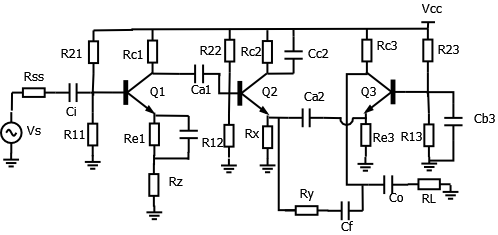
\includegraphics[width=0.75\linewidth]{img/CircuitoComRealimenta.png}
\caption{Esquema eletrônico do circuito com os resistores indicados}
Fonte: Autoria própria
\label{fig:circuito1}
\end{figure}

Os valores de resistência comerciais de resistências utilizados no circuito da figura \ref{fig:circuito1} estão descritos a seguir:

$ R_{b1} = R_{21}//R_{11} = 100 k\Omega$

$R_{e1} = 560 \Omega$

$R_{c1} = 2,7 k\Omega$

$R_{SS} = 50 \Omega$

$ R_{b2} = R_{22}//R_{12} = 100 k\Omega$

$R_{x} = 560 \Omega$

$R_{c2} = 2,7 k\Omega$

$ R_{b3} = R_{21}//R_{11} = 100 k\Omega$

$R_{e3} = 560 \Omega$

$R_{c3} = 2,7 k\Omega$

$R_{y} = 56 k\Omega$

$R_{L} = 1,5 k\Omega$


Os capacitores comerciais utilizados no circuito da figura \ref{fig:circuito1} estão determinados a seguir:

$C_i = 4,7  \mu F$

$C_o = 1 \mu F$

$C_{a1} = 1 \mu F$

$C_{a2} = 220 \mu F$

$C_{e1} = 470 \mu F$

$C_{a1} = 1 \mu F$

$C_{b3} = 98,3 nF$

$C_{c2} = 1,3 \mu F$


\section{Parâmetros dos transístores}
\label{sec:par_trans}

Foram utilizados três transístores BC639 cuja pinagem está descrita na figura \ref{fig:bc_639}. Foram medidos os parâmetros hfe e hie descritos na sequência.

\begin{figure}[H]
\centering
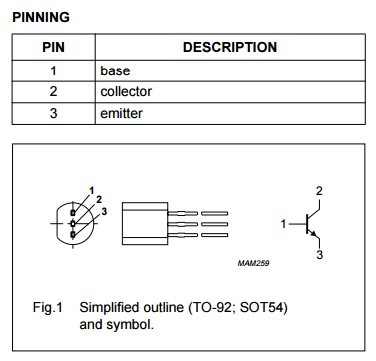
\includegraphics[width=0.75\linewidth]{img/BC639.png}
\caption{Transístor BC639}
Fonte: Philips
\label{fig:bc_639}
\end{figure}

$hfe_1 = 248$

$hfe_2= 256$

$hfe_3 = 255$

$hie_1= 1,735 k\Omega$

$hie_2= 1,784 k\Omega$

$hie_3= 1,777 k\Omega$


\section{Polarização DC de Transistores bipolares}
\label{sec:dim_trans}

Nesta seção foi dimensionado os resistores de polarização de modo que o transistor opere na região linear. Para isso foi utilizado o seguinte método:

Primeiramente, foi fornecida a informação que a fonte $V_{cc}$ deveria ser de $30 V$ e que o transítor para os três estágio deveria ser BC639.

Escolheu-se o valor de $I_C$ que é $80 mA$.

O fator de estabilidade foi determinado como sendo 5, pois a faixa de valores ótimos está compreendida entre $1 \leq S \leq 10$, o valor ideal
teórico seria 1, mais isto implicaria em valores muito baixos para os resistores $R_1$ e $R_2$,
tendo como conseqüência um consumo maior de energia da fonte DC.

Cálculo de $R_C$:

\begin{equation}
( R_c + R_e ) \approx \frac{V_{cc} - V_{ce}}{I_c}
\end{equation}

O valor obtido $( R_c + R_e )$ é aproximadamente o valor de $R_c$, pois o valor nominal de $R_e$ é muito pequeno comparado com $R_c$. Logo, escolhe-se o valor comercial de $R_c$ abaixo do encontrado no resultado acima.

% * <jessicasampaio@alunos.utfpr.edu.br> 2016-04-11T04:21:36.281Z:
%
% colocar tabela de resistores comerciais equivalentes
%
% ^.

Para calcular $R_e$ utiliza-se o gráfico para determinar hfe. Com isso, calcula-se $R_e$ a partird da malha coletor emissor e da expressão para $I_e$ \ref{eq:malha_emissor_e_Ie}. Chega-se na equação \ref{eq:expr_Re}. Assim, o valor de $R_e$ foi determinado e escolhe-se um
valor comercial de Re um pouco acima do calculado de modo que Ic será menor. 
% * <jessicasampaio@alunos.utfpr.edu.br> 2016-04-11T04:22:32.609Z:
%
% colcar a referencia a tabela de resistores
%
% ^.

\begin{equation}\label{eq:malha_emissor_e_Ie}
V_{CC} = V_{R_C} + V_{C_E} + V_{R_E}  \therefore  I_e =\frac{I_c \left(hfe + 1 \right)}{hfe}
\end{equation}

\begin{equation}
VCC = R_c\cdot I_c + V_{C_E} + R_e \cdot I_e
\end{equation}

\begin{equation}\label{eq:expr_Re}
R_e = \frac{Vcc - V_{C_E} - R_c \cdot I_c}{I_c \cdot \left[ \frac{\left(hfe + 1 \right)}{hfe} \right]}
\end{equation}

% * <jacichen@alunos.utfpr.edu.br> 2016-04-11T03:59:28.888Z:
%
% > !!!
%
% Que grafico?
%
% ^ <jessicasampaio@alunos.utfpr.edu.br> 2016-04-11T04:23:20.672Z:
%
% Encontrar um gráfico na internet de Vbe por Ic referente a esse transístor
%
% ^.

\begin{equation}
S = \left(hfe + 1 \right)\frac{1 + \left( \frac{R_b}{R_e} \right)}{\left(hfe + 1 \right) + \left(\frac{R_b}{R_e} \right)}
\end{equation}

\begin{equation}
R_b = \frac{ \left(hfe + 1 \right) \cdot \left( S - 1 \right)}
{(hFE + 1 ) - S}
\end{equation}

Recálculo de Ic em função dos valores comerciais adotados para Rc e Re:

\begin{equation}
I_c = \frac{V_{CC} - V_{CE}}{R_C-R_E \cdot \frac{hfe+1}{hfe}}
\end{equation}

\begin{equation}
V_{th} = R_{th} \cdot I_B + V_{be} + R_E I_E = R{th} \frac{I_C}{hfe} + V_{BE} + R_E \cdot\left(\frac{I_C\left(hfe+1\right)}{hfe}\right)
\end{equation}

\begin{equation}
V_{th} = \frac{R_2}{R_1+R_2} \cdot V_{CC}
\end{equation}

\begin{equation}
R_{th} = \frac{R_1\cdot R_2}{R_1 + R_2}
\end{equation}

\begin{equation}
\frac{V_{th}} {V_{CC}} = \frac{R_2}{R_2+R_1}
\end{equation}

\begin{equation}
R_1 = R_{th} \cdot \frac{V_{th}} {V_{CC}}
\end{equation}

\begin{equation}
R_2 = \frac{R_{th} \cdot R_1}{ R_B - R_1}
\end{equation}

\begin{equation}
B_{BB}  = \frac{R_2 \cdot V_{CC}}{ R_1 \cdot R_2}
\end{equation}

\begin{equation}
I_C = \frac{hfe \cdot \left(V_{BB} - V_{be}\right)}{R_b + R_e \cdot \left(hfe+1\right)}
\end{equation}

\begin{equation}
V_{ce} = V_{cc} - R_c \cdot I_c - R_e \cdot I_c \cdot \left[ \frac{hfe +1 }{hfe} \right]
\end{equation}

Os valores de polarização determinados teoricamente a partir dos parâmetros dos transístores, da seção \ref{sec:dim_trans}, é exibido na tabela \ref{tab:pol_teorica} a seguir:

\begin{table}[H]
\centering
\caption{Valores de polarização do circuito teórico}
\label{tab:pol_teorica}
\begin{tabular}{|ll|ll|ll|}
\hline
$I_{B_{EC}}$  & $14,83\mu A$  & $I_{B_{CC}}$  & $14,38\mu A$  & $I_{B_{BC}}$  & $14,43\mu A$  \\ \hline
$I_{C_{EC}}$  & $3,68 mA$ & $I_{C_{CC}}$  & $3,68 mA$ & $I_{C_{BC}}$  & $3,68  mA$ \\ \hline
$V_{CE_{EC}}$ & $17,98V$      & $V_{CE_{CC}}$ & $17,98V$      & $V_{CE_{BC}}$ & $17,98V$      \\ \hline
\end{tabular}
\end{table}

\section{Dimensionamento dos Capacitores}

Os capacitores foram dimensionados a partir das resistências equivalentes vistas por eles no circuito. A seguir  é mostrado como foi calculado as capacitâncias para uma frequência $f_L$ igual a $300 Hz$, adimitindo-se que o capacitor dominante é o $C_{b3}$, cuja resistência equivalente é a menor de todas. Os resultados encontram-se na tabela \ref{tab:capacitores}.

	Primeiramente, equaciona em \ref{eq:fL} a frequência de corte nas baixas frequências, isto é, $f_L$ com os respectivos capacitores que o circuito deve ter.

\begin{equation}\label{eq:fL}
f_L = \frac{1}{2 \cdot \pi} \cdot \left( \frac{1}{C_i \cdot R_{eqi}} + \frac{1}{C_o \cdot R_{eqo}} + \frac{1}{C_{a1} \cdot R_{eqa1} }+ \frac{1}{C_{a2} \cdot R_{eqa2}} +\frac{1}{C_{b3} \cdot R_{eqb3}} + \frac{1}{C_{e1}\cdot R_{eqe1}} + \frac{1}{C_{c2}\cdot R_{eqc2}} \right)
\end{equation}

	Multiplica-se toda a equação \ref{eq:fL} por $2 \cdot \pi$ para obter-se a frequência ângular.

\begin{equation}
w_L = w_i + w_o + w_{a1} + w_{a2} + w_{b3} + w_{e1} + w_{c2}
\end{equation}

Multiplicando todos os capacitores a não ser o dominante por um fator de 10x:
\begin{equation}
w_L = \frac{w_cal}{10}+\frac{w_cal}{10}+\frac{w_cal}{10}+\frac{w_cal}{10}+ w_{cal} +\frac{w_cal}{10} +\frac{w_cal}{10}
\end{equation}

Sendo $w_L = 2 \cdot \pi f_L = 1885 [rad/s]$ obtem-se a frequência de cálculo que é $w_{cal} = 2693 [rad/s]$. Logo todos os capacitores a não ser o dominante podem ser calculados com a equação \ref{eq:deter_cap} . O capacitor dominante é dado pela equação \ref{eq:deter_cap_dom}.

\begin{equation}\label{eq:deter_cap}
C_{indice} = \frac{10}{w_{cal} \cdot R_{eq\left(indice\right)}}
\end{equation}


\begin{equation}\label{eq:deter_cap_dom}
C_{indice} = \frac{1}{w_{cal} \cdot R_{eq\left(indice\right)}}
\end{equation}

\begin{table}[H]
\centering
\caption{Valores dos capacitores teóricos}
\label{tab:capacitores}
\begin{tabular}{|l|l|}
\hline
$C_{a1} u[F]$ & 1    \\ \hline
$C_{a2} u[F]$ & 210  \\ \hline
$C_{i} u[F]$  & 3,8  \\ \hline
$C_{b3} n[F]$ & 98,3 \\ \hline
$C_{o} u[F]$  & 1    \\ \hline
$C_{e1} u[F]$ & 530  \\ \hline
$C_{c2} u[F]$ & 1,3  \\ \hline
\end{tabular}
\end{table}



\section{Equações de ganho}
\label{sec:eq_ganho}

\subsection{Ganho sem Realimentação com efeito de carga}
\label{subsec:sem_real}
Determinou-se o ganho do sistema separando o amplificador com realimentação em dois blocos, o amplificador básico A e o circuito de realimentação $\beta$. Dessa maneira, é calculado as características importantes do sistema com realimentação a partir de A e $\beta$, isto é, os valores $A_f$, $R_{i_f}$ e $R_{o_f}$. 

Nesta análise, o circuito da figura \ref{fig:circuito1} foi modificado para o circuito 


\begin{figure}[H]
\centering
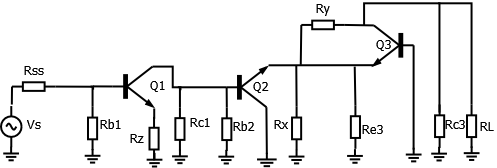
\includegraphics[width=0.75\linewidth]{img/CircuitoComRealimentaoSinal.png}
\caption{Equivalente para o sinal do circuito da figura \ref{fig:circuito1} com realimentação}
Fonte: Autoria própria
\label{fig:circuito_sinal_com_real}
\end{figure}


\begin{figure}[H]
\centering
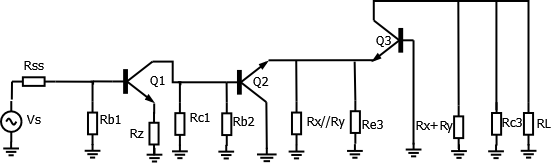
\includegraphics[width=0.75\linewidth]{img/CircuitoSemRealimentaoSinal.png}
\caption{Equivalente para o sinal do circuito da figura \ref{fig:circuito1} com efeito de carga do elo de realimentação}
Fonte: Autoria própria
\label{fig:circuito_sinal_sem_real}
\end{figure}


Os estágios 2 e 3 do circuito apresentam uma realimentação compartilhada entre o coletor do terceiro estágio e o emissor do segundo estágio, portanto, analisou-se a configuração amplificador básico desses estágios separados do primeiro estágio, o qual possui sua realimentação no emissor.
	As próximas subseções \ref{subsec:stage_2_3} e \ref{subsec:stage1} abordarão essa análise.

\subsection{Estágios CC e BC}
\label{subsec:stage_2_3}

Primeiramente, obteve-se a configuração do amplificador básico para os estágios 2 e 3, sem realimentação mas levando em conta a influência de $\beta$ no circuito através da análise da topologia que esses estágios possuem.

A topologia apresentada pelos estágios 2 e 3 é a série de tensão, logo é aplicado o método adequado para a análise desse amplificador realimento \cite{millman}.Primeiro, determina-se o circuito de entrada fazendo $V_o = 0$ para a amostragem de tensão. Em outras palavras, curto-circuitar o nó de saída. Em seguida, determina-se o circuito de saída fazendo $I_i = 0$ para a configuração séria, ou seja, deve-se abrir a malha de entrada da realimentação. A figura \ref{fig:AnaliseEstagio23}
mostra o amplificador dos estágios 2 e 3 sem relimentação mas com o efeito da carga que o elo de realimentação produz.

\begin{figure}[H]
\centering
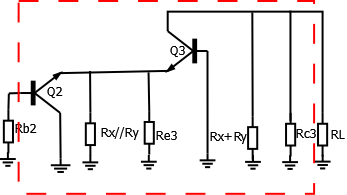
\includegraphics[width=0.75\linewidth]{img/AnaliseEstagio23.png}
\caption{Circuito equivalente sem realimentação mas com efeito de carga do elo de realimentação para os estágios 2 e 3}
Fonte: Autoria própria
\label{fig:AnaliseEstagio23}
\end{figure}

Através do circuito  \ref{fig:AnaliseEstagio23} foi determinado o ganho de tensão para cada estágio, através da fórmula \ref{eq:ganho_tensao}. Os ganhos encontrados para o circuito coletor comum e base comum, são repectivamente os expressos pelas fórmulas \ref{eq:Av_coletor_comum} e \ref{eq:Av_base_comum}.

\begin{equation}\label{eq:ganho_tensao}
A_{v} = \frac{v_o}{v_i}
\end{equation}


\begin{equation}\label{eq:Av_base_comum}
A_{V_{bc}}= \frac{hfe}{hie} \left(\left(R_{x}+R_{y}\right)//R_{c_3}\right)
\end{equation}

\begin{equation}\label{eq:Av_coletor_comum}
A_{V_{cc}}= \frac{hfe \left(R_x//R_y//R_{E_3}\right)}{hie+hfe\left(R_x//R_y//R_{E_3}\right)} 
\end{equation}


O ganho de tensão total desse sistema é expresso em \ref{eq:Av_total_CC_BC}.

\begin{equation}\label{eq:carga_est2}
R_{L_2}'=R_x//R_y//R_{E_3}
\end{equation}

\begin{equation}\label{eq:carga_est3}
R_{L_3}'=\left(R_{x}+R_{y}\right)//R_{c_3}
\end{equation}

\begin{equation}\label{eq:Av_total_CC_BC}
A_{V_{t_1}} = \frac{hfe R_{L_2}'}{hie+hfe R_{L_2}'}  \frac{hfe}{hie} R_{L_3}'
\end{equation}

O fator de transmissão reverso foi determinado em \ref{eq:fator_trans_inverso1}

\begin{equation}\label{eq:fator_trans_inverso1}
\beta{_1} = \frac{x_f}{x_o} = \frac{V_f}{V_o} = \frac{R_X}{R_x+R_y}
\end{equation}

A dissensibilidade foi determinada em \ref{eq:dissensibilidade1}

\begin{equation}\label{eq:dissensibilidade1}
D_1 = 1+ \beta{_1} A_{V_{t_1}}
\end{equation}

Logo, o ganho com realimentação foi determinado através da equação expressão \ref{eq:Avf1}.

\begin{equation}\label{eq:Avf1}
A_{vf} = \frac{A_{V_{t_1}}}{D_1}
\end{equation}


A impedância de entrada do segundo estágio sem reaalimentação mas com o efeito da carga de $\beta$ é dado pela equação \ref{eq:resistencia_i_1}, e com realimentação é dado pela equação \ref{eq:resistencia_if_1}. A resistência de saída sem realimentação mas com o efeito da carga de $\beta$ é expresso pela equação \ref{eq:resistencia_o_1} e com realimentação pela equação \ref{eq:resistencia_of_1}.

\begin{equation} \label{eq:resistencia_i_1}
R_i =hie_2+\left(hfe_2+1\right)\cdot\left(R_x//R_y\right)//R_{e3}//\frac{hie_3}{hfe_3+1}
\end{equation}



\begin{equation}\label{eq:resistencia_o_1}
R_o =\left(R_x+R_y\right)//R_{c3}
z\end{equation}



\begin{equation}\label{eq:resistencia_if_1}
R_{if} =Ri\cdot D
\end{equation}


\begin{equation}\label{eq:resistencia_of_1}
R_{of} = \frac{R_o}{D}
\end{equation}

\subsection{Estágio EC}
\label{subsec:stage1}
O primeiro estágio (emissor comum) redesenhado em termos de sinal e sem realimentação é expresso pela figura \ref{fig:sinal_estagio1}.



\begin{figure}[H]
\centering
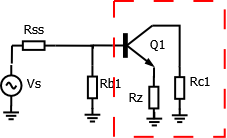
\includegraphics[width=0.75\linewidth]{img/SinalEstagio1.png}
\caption{Equivalente para o sinal do estágio 1 \ref{fig:circuito1} sem realimentação mas com o efeito da carga do elo de realimentação}
Fonte: Autoria própria
\label{fig:sinal_estagio1}
\end{figure}


O ganho do primeiro estágio considerando a saída em aberto é dado pela expressão , quando o limite de $R_L$ tende a infinito em relação a $A_V$ expresso pela equação \ref{eq:ganho_aberto_estagio1}.



\begin{equation}\label{eq:carga_st1}
R_{L_1}'=\left(R_{c_1}//R_{b_2}\right)//hie_2+\left(Rx//R_y//R_{e3}\right)\left(hfe+1\right) 
\end{equation}

\begin{equation}\label{eq:Av_emissor_comum}
A_{V_{e}}= \frac{hfe}{hie} \left(R_{c_1}//R_{b_2}\right)//hie_2+\left(Rx//R_y//R_{e3}\right)\left(hfe+1\right) 
\end{equation}


\begin{equation} \label{eq:ganho_aberto_estagio1}
A_{ve}= \lim_{R_L->\infty} A_{V_{e}}
\end{equation}

O fator de dissenssibilidade é calculado como:

\begin{equation}
D= 1+ \beta \cdot A_{Ve}
\end{equation}

\begin{equation}
A_{vf_{ec}} = \frac{A_{V_{ec}}}{D_{ec}}  
\end{equation}

A impedância de entrada desse estágio sem reaalimentação mas com o efeito da carga de $\beta$ é dado pela equação \ref{eq:resistencia_i_2}, e com realimentação é dado pela equação \ref{eq:resistencia_if_2}. A resistência de saída sem realimentação mas com o efeito da carga de $\beta$ é expresso pela equação \ref{eq:resistencia_o_2} e com realimentação pela equação \ref{eq:resistencia_of_2}.

\begin{equation} \label{eq:resistencia_i_2}
R_i = hie_1 + R_z \cdot (hfe_1+1)
\end{equation}



\begin{equation}\label{eq:resistencia_o_2}
R_o = R_{c1} + R_z \cdot (hfe+1)
z\end{equation}



\begin{equation}\label{eq:resistencia_if_2}
R_{if} =R_i\cdot D
\end{equation}


\begin{equation}\label{eq:resistencia_of_2}
R_{of} = \frac{R_o}{D}
\end{equation}


\begin{figure}[H]
\centering
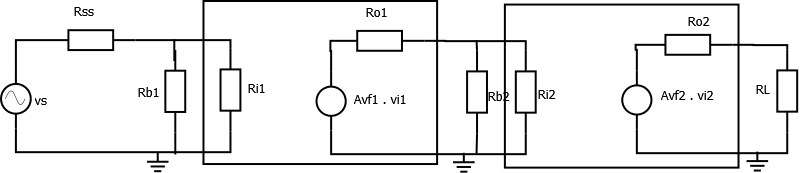
\includegraphics[width=0.75\linewidth]{img/CircuitoRealimentacaoTensaoSerieResistencias.png}
\caption{Circuito com realimentação série de tensão com as resistências de entrada e saída indicados}
Fonte: Autoria própria
\label{fig:circuito_real_resistencia}
\end{figure}


\section{Análise em Frequêcia}
\label{sec:ana_freq}

A análise da resposta em frequência do amplificador construído seguirá os métodos descritos em \citeonline{pedroni}, ou seja, será dividida a análise em baixa frequência e em alta frequência, para o circuito com realimentação e para o circuito com o efeito da carga do elo de realimentação. 
\subsection{Análise em baixa frequência}



\subsubsection{Circuito com Realimentação}
A função de transferencia em médias e baixas frequências para o circuito da figura \ref{fig:circuito1} é dada pela equação \ref{eq:freq_b_m_real}. Existem 5 zeros em $w=0$ responsáveis pelo acoplamento do sinal. Também existem três zeros em $\omega = \frac{1}{R.C}$ são referentes aos três capacitores de desacoplamento do sinal(onde $R$ é o valor da resistência desacoplada).Por fim, cada capacitor apresenta um pólo para $\omega = \frac{1}{R_{eq}.C}$ originário do equivalente de Thévenim para os respectivos capacitores. Substituindo os valores pelos encontrados nas tabelas
% * <jessicasampaio@alunos.utfpr.edu.br> 2016-04-11T04:16:51.001Z:
%
% indicar tabelas onde os valores se encontram bem como as equações referentes a eles
%
% ^.

\begin{equation}\label{eq:freq_b_m_real}
A_{VS}(s) = A_{VS} \frac{w^5 \cdot \left(s+\frac{1}{R_{e1}\cdot C_{e1}}\right)\cdot \left(s+\frac{1}{R_{c2}\cdot C_{c2}}\right)\cdot \left(s+\frac{1}{R_{b3}\cdot C_{b3}}\right)}{\left(s+\omega_i\right)\left(s+\omega_{a1}\right)\left(s+\omega_o\right)\left(s+\omega_{e1}\right)\left(s+\omega_{a2}\right)\left(s+\omega_{b3}\right)\left(s+\omega_{c2}\right)\left(s+\omega_{f}\right)}
\end{equation}
% * <jessicasampaio@alunos.utfpr.edu.br> 2016-04-11T04:14:24.268Z:
%
% Falta calcular os polos equivalentes
%
% ^.
\begin{equation}\label{eq:freq_b_m_real}
A_{VS}(s) = A_{VS}\frac{w^5 \cdot \left(s+\frac{1}{R_{e1}\cdot C_{e1}}\right)\cdot \left(s+\frac{1}{R_{c2}\cdot C_{c2}}\right)\cdot \left(s+\frac{1}{R_{b3}\cdot C_{b3}}\right)}{\left(s+\omega_i\right)\left(s+\omega_{a1}\right)\left(s+\omega_o\right)\left(s+\omega_{e1}\right)\left(s+\omega_{a2}\right)\left(s+\omega_{b3}\right)\left(s+\omega_{c2}\right)\left(s+\omega_{f}\right)}
\end{equation}

\subsubsection{Circuito com efeito de carga do elo de realimentação}

A função de transferência para médias e baixas frequÊncia para o circuito com efeito de carga do elo de realimentação é dada pela equação \ref{eq:freq_b_m_sem_real}. Os 4 zeros dados por $w = 0$ referen-se aos capacitores de acoplamento do sinal. Os três zeros devido a  $\omega = \frac{1}{R.C}$ referen-se aos capacitores de desacoplamento, onde R é o resistor desacoplado. Para os pólos, $\omega = \frac{1}{R_{eq}.C}$ para cada capacitor presente no circuito.


\begin{equation}\label{eq:freq_b_m_sem_real}
A_{VS}(s) = A_{VS}\frac{s^4 \cdot \left(s+\frac{1}{R_{e1}\cdot C_{e1}}\right)\cdot \left(s+\frac{1}{R_{c2}\cdot C_{c2}}\right)\cdot \left(s+\frac{1}{R_{b3}\cdot C_{b3}}\right)}{\left(s+\omega_i\right)\left(s+\omega_{a1}\right)\left(s+\omega_o\right)\left(s+\omega_{e1}\right)\left(s+\omega_{a2}\right)\left(s+\omega_{b3}\right)\left(s+\omega_{c2}\right)}
\end{equation}

\begin{equation}\label{eq:freq_b_m_sem_real}
A_{VS}(s) = A_{VS} \frac{s^4 \cdot \left(s+\frac{1}{R_{e1}\cdot C_{e1}}\right)\cdot \left(s+\frac{1}{R_{c2}\cdot C_{c2}}\right)\cdot \left(s+\frac{1}{R_{b3}\cdot C_{b3}}\right)}{\left(s+\omega_i\right)\left(s+\omega_{a1}\right)\left(s+\omega_o\right)\left(s+\omega_{e1}\right)\left(s+\omega_{a2}\right)\left(s+\omega_{b3}\right)\left(s+\omega_{c2}\right)}
\end{equation}



\subsection{Análise em alta frequência}

\subsection{Circuito Realimentado}
A análise em alta frequência do circuito exigiu o calculo das capacitância intrínsecas dos transistores considerados. Foi consultado o manual do fabricante do transístor BC639, em que o valor de $C_{ob}$ é fornecido. Este valor corresponde aproximadamente ao valor de $C_\mu$.

Com isso, foi determinado a capacitância $C_\pi$ a partir da frequência de transição $f_T$ e de $C_\mu$ através da equação \ref{eq:freq_trans}. 

\begin{figure}[H]
\centering
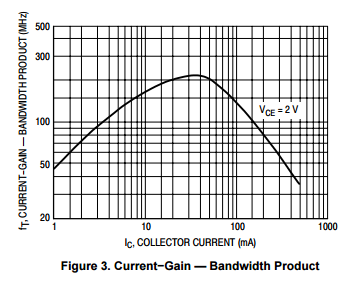
\includegraphics[width=0.75\linewidth]{img/bandwith_product_ft.png}
\caption{$f_T$ a partir de $I_C$}
Fonte: SCILLC
\label{fig:fT_apartid_IC}
\end{figure}

A frequência de transição foi determinada como sendo $100 MHz$ a partir da do gráfico \ref{fig:fT_apartid_IC})  e do valor de $I_C$ determinado na seção \ref{sec:dim_trans}. Foi necessário também calcular gm dado pela equação \ref{eq:gm}.



\begin{equation}\label{eq:gm}
gm \approx 39 \cdot I_C
\end{equation}


\begin{equation} \label{eq:freq_trans}
f_T = \frac{gm}{2 \cdot \left(C_{\mu} + C_{\pi}\right)}
\end{equation}

Os valores encontrados foram: $C_\mu = 7 pF$ e $C_\pi = 221 pF $ para $f_T = 100 M Hz$, $gm = 143,52 m s$ e $I_C = 3,68 mA$

A função de transferência agora pode ser determinada analisando o circuito \ref{fig:circuito1} em altas frequências, isto é, cada estágio é substituido pelo seu modelo equivalente para alta frequência.

O pólo dominante do primeiro, segundo e terceiro estágios são respectivamente os expressos nas equações
\ref{eq:polo1}, \ref{eq:polo2} e \ref{eq:polo3}. Observa-se nessas equações que podemos obter uma solução com erro aceitável, para efeito de estimativa dos pólos de alta frequência do circuito, a não interação dos pólos do primeiro com os do segundo estágio, e os do terceiro estágio \cite{millman}.


\begin{equation}\label{eq:polo1}
p_1 = \frac{1}{ \left[r_{\pi}//\left(r_x+ R_S//R_{b1}\right)\right]   
\cdot \left(C_\pi+g_m \cdot   \left(R_{c1}//R_z \cdot \left(\frac{hfe_1+1}{hfe_1}\right)  //R_{b2}//hie_2 + Rx \cdot \left( hfe_2 + 1 \right) \right) \cdot C_{\mu}\right)}
\end{equation}



\begin{equation}\label{eq:polo2}
p_2 = \frac{gm \cdot \left( R_x//R_y//R_{e3} + hie_3 \left(hfe_3+1\right)\right) }{r_x+ R_c1 + R_z \cdot \left(hfe_1+1\right) \cdot \left( C_{\pi} + gm \cdot \left( R_x//R_y//R_{e3} + hie_3 \cdot \left(hfe_3+1\right)\right)  \cdot C_{\mu}\right)}
\end{equation}


\begin{equation}\label{eq:polo3}
p_3 = \frac{gm \cdot g_x \cdot G'_L \cdot G'}{\left(gm \cdot G''+ g_x \cdot G'\right) \cdot gm \cdot C_{\mu} +\left(gm \cdot G'''+ g_x \cdot G'\right) \cdot G'_L \cdot C_{\pi}}
\end{equation}

G', G'' e G''' são dados pelas equações \ref{eq:G1}, \ref{eq:G2} e \ref{eq:G3}.

\begin{equation}\label{eq:G1}
G'= gm+G_E+G_s
\end{equation}


\begin{equation}\label{eq:G2}
G''= G_E+G_s + G'_L
\end{equation}


\begin{equation}\label{eq:G3}
G'''= g_x+G_E+G_s
\end{equation}



\section{Ensaio efetuado}
\label{sec:ensaio}
Para o primeiro emperimento, depois de ser projetado o circuito foi seguido o seguinte roteiro de execução de ensaios: experimentos com circuitos sem realimentação, experimentos com circuito com efeito de carga e experimento com circuito realimentado. O sinal base para estas medições foi de $100mV$ com frequência de $10kHz$. Quando os sinais se tornavam destorcidos demais por causa do corte/saturação do transistor, utilizou-se um atenuador de -23dB na entrada.

Mediu-se primeiramente os valores de polarização do circuito sem realimentação. Anotou-se os valores dos resistores e capacitores medidos, com a ponte RLC e o multímetro. Em seguida, foi conferido as frequências de corte inferior e superior.

Em seguida, foi utilizado o circuito sem realimentação, mas com efeito de carga. Nele, foram medidos impedância de entrada e saída, o ganho apropriado ao circuito e a resposta em frequência, retirando-se 20 pontos para construir o diagrama de bode e incluindo os pontos de meia potência (frequência de corte).

Para o circuito realimentado, foram realizadas as mesmas medições (impedâncias, ganho e resposta em frequência). Por fim, foi aumentado a realimentação até que o circuito entra-se em instabilidade. Se não fosse possível isso, seria anotado o valor máximo de  realimentação. Se ele entrasse em instabilidade, deveria-se tentar modificar o pólo em alta para compensá-lo.

Para o segundo experimento, foi montado o circuito da figura \ref{fig:exp2}. $Q_1$ e $Q_2$ são os transistores TIP32 e TIP31, respectivamente. O amplificador exibido é o \textit{amp-op} LM741. 

\begin{figure}[H]
\centering
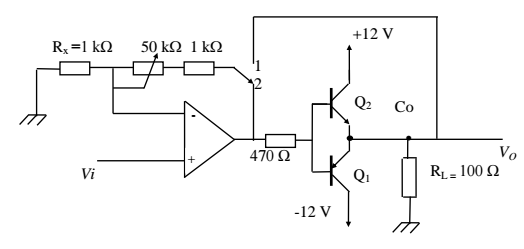
\includegraphics[width=0.8\linewidth]{img/exp2.png}
\caption{Segundo experimento realizado}
Fonte: Fornecido pelo professor
\label{fig:exp2}
\end{figure}

Nele, foram realizadas comparações dos sinais na saída do amplificador opercional e da saída dos TIP's (em $R_L$) em dois momentos distintos: primeiramente quando a chave estava na posição 2, e em seguida com a chave na posição 1. O valor de realimentação foi sendo modificado através do potenciômetro e os sinais de saída descrito poderam ser analisados. O sinal aplicado foi de $100mV$ e $1kHz$.

%--------------terceiro capitulo----------
\chapter{Resultados e Discussões} 
\label{sec:anal_dados}

\section{Amplificador de três estágios (Primeiro experimento)}



\subsection{Polarização}

Os resultados obtidos para a polarização medidos no circuito sem realimentação e efeito de carga encontram-se na tabela \ref{tab:pol_pratica}.

\begin{table}[H]
\centering
\caption{Valores de polarização do circuito medido}
\label{tab:pol_pratica}
\begin{tabular}{|ll|ll|ll|}
\hline
$I_{B_{EC}}$  & $17,4\mu A$  & $I_{B_{CC}}$  & $17,4\mu A$  & $I_{B_{BC}}$  & $17,6\mu A$  \\ \hline
$I_{C_{EC}}$  & $3,75 mA$ & $I_{C_{CC}}$  & $3,71 mA$ & $I_{C_{BC}}$  & $3,76 mA$ \\ \hline
$V_{CE_{EC}}$ & $18,0V$      & $V_{CE_{CC}}$ & $17,8V$      & $V_{CE_{BC}}$ & $17,7V$      \\ \hline
\end{tabular}
\end{table}

Os valores encontrados são sólidos e condizentes com o esperado.

\subsection{Ganho de tensão}
\label{sec:ganho_tensao_transc}
O ganho de tensão para o amplificador sem realimentação foi de 1235 (utilizando o atenuador de $-23dB$, sendo mais do que o suficiente encontrado para realizar o experimento.

\subsection{Impedâncias}
As impedâncias de entrada e saída encontradas (utilizando o método de divisor de corrente), para $Z_i$ e $Z_o$ são $1,84k\Omega$ com $3,77k\Omega$ para o circuito apenas efeito de carga, sem realimentação; e $1,92k\Omega$ com $2,36k\Omega$ para o circuito realimentado.

\subsection{Resposta em frequência}
Os pólos de baixa e alta frequência encontrados no circuito sem realimentação foram $110Hz$ e $950kHz$, respectivamente, o que é uma boa faixa para evitar o efeito de instabilidade. 

\begin{table}[H]
\centering
\caption{Resposta em frequência sem realimentação mas com efeito de carga}
\label{tab:resp_freq_sem_realimentacao}
\begin{tabular}{ | l | l | l | }
\hline
	Frequências & Av & Fase \\ \hline
	10 & 12.5424 & -4 \\ \hline
	25 & 100.5 & -9 \\ \hline
	40 & 229.14 & -45 \\ \hline
	55 & 337.68 & -66 \\ \hline
	70 & 426.12 & -82 \\ \hline
	100 & 562.8 & -107 \\ \hline
	180 & 694.65 & -130 \\ \hline
	250 & 739.68 & -145 \\ \hline
	500 & 836.16 & -160 \\ \hline
	750 & 900.48 & -160 \\ \hline
	1000 & 892.44 & -160 \\ \hline
	5000 & 1069.32 & -175 \\ \hline
	10000 & 1065.3 & -180 \\ \hline
	50000 & 1061.28 & 180 \\ \hline
	100000 & 1061.28 & 180 \\ \hline
	250000 & 1045.2 & 160 \\ \hline
	500000 & 980.88 & 145 \\ \hline
	750000 & 884.4 & 130 \\ \hline
	1000000 & 771.84 & 110 \\ \hline
	1500000 & 578.88 & 80 \\ \hline
	2000000 & 418.08 & 70 \\ \hline
	3000000 & 225.12 & 45 \\ \hline
\end{tabular}
\end{table}

\begin{figure}[H]
\centering
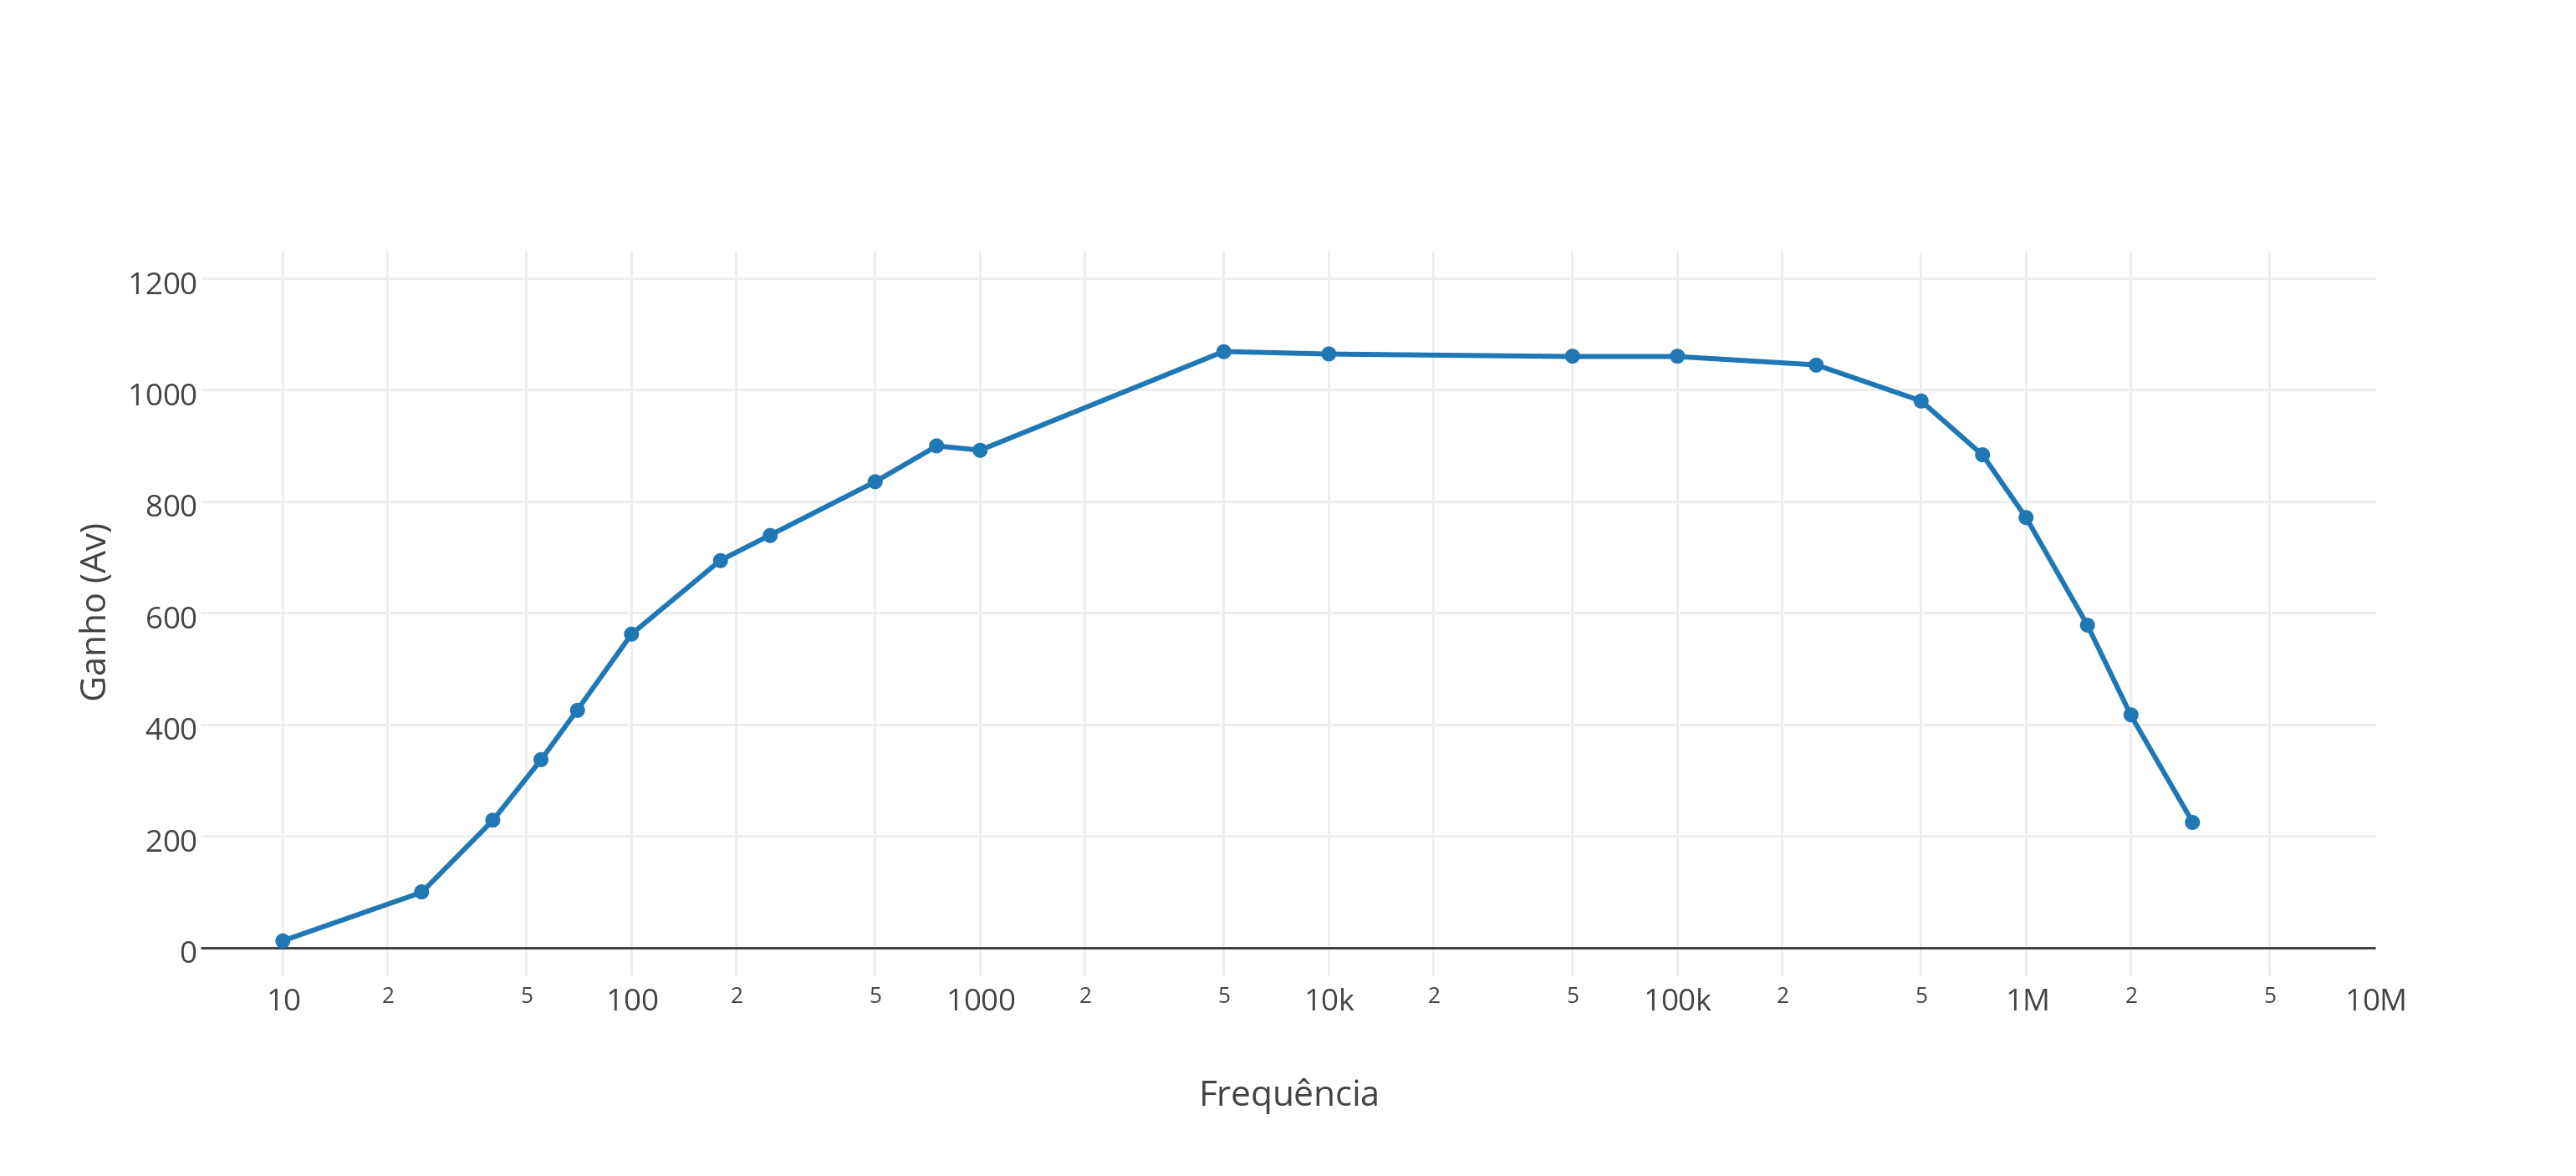
\includegraphics[width=0.8\linewidth]{img/Projeto2_SemRealimentac_a_o.png}
\caption{Resposta em frequência (ganho) sem realimentação mas com efeito de carga}
\label{fig:resp_freq_sem_real_fase}
\end{figure}

\begin{figure}[H]
\centering
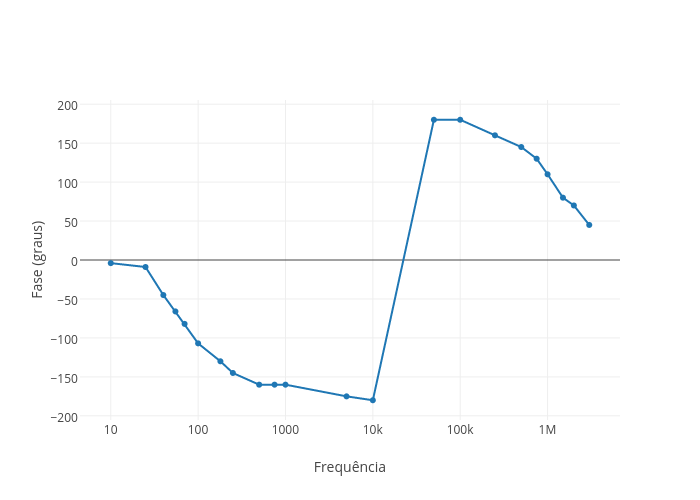
\includegraphics[width=0.8\linewidth]{img/SemReal_Fase.png}
\caption{Resposta em frequência (fase) sem realimentação mas com efeito de carga}
\label{fig:resp_freq_sem_real_fase}
\end{figure}

\begin{table}[H]
\centering
\caption{Resposta em frequência com realimentação}
\label{tab:resp_freq_com_realimentacao}
\begin{tabular}{ | l | l | l | }
\hline
	Frequência(Hz) & Av & Fase \\ \hline
	10 & 1.25 & -4 \\ \hline
	25 & 23 & -9 \\ \hline
	40 & 51.47 & -45 \\ \hline
	55 & 69.18 & -66 \\ \hline
	70 & 114.84 & -82 \\ \hline
	100 & 126.74 & -107 \\ \hline
	180 & 146.97 & -130 \\ \hline
	250 & 155.52 & -145 \\ \hline
	500 & 166.66 & -160 \\ \hline
	750 & 187.17 & -160 \\ \hline
	1000 & 217.83 & -160 \\ \hline
	5000 & 226.80 & -175 \\ \hline
	10000 & 229.76 & -180 \\ \hline
	50000 & 230.26 & 180 \\ \hline
	100000 & 241.14 & 180 \\ \hline
	250000 & 229.16 & 160 \\ \hline
	500000 & 212.56 & 145 \\ \hline
	750000 & 198.64 & 130 \\ \hline
	1000000 & 168.43 & 110 \\ \hline
	1500000 & 127.16 & 80 \\ \hline
	2000000 & 89.86 & 70 \\ \hline
	3000000 & 48.24 & 45 \\ \hline
\end{tabular}
\end{table}

\begin{figure}[H]
\centering
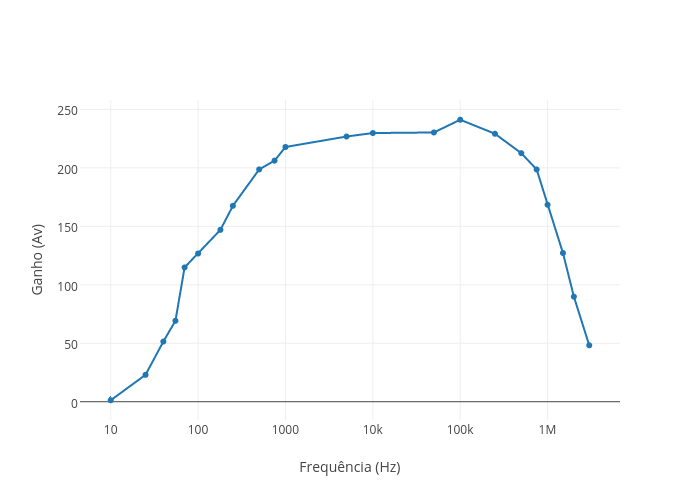
\includegraphics[width=0.8\linewidth]{img/RespFreq_ComReal.png}
\caption{Resposta em frequência com realimentação}
\label{fig:resp_freq_com_real}
\end{figure}

\begin{figure}[H]
\centering
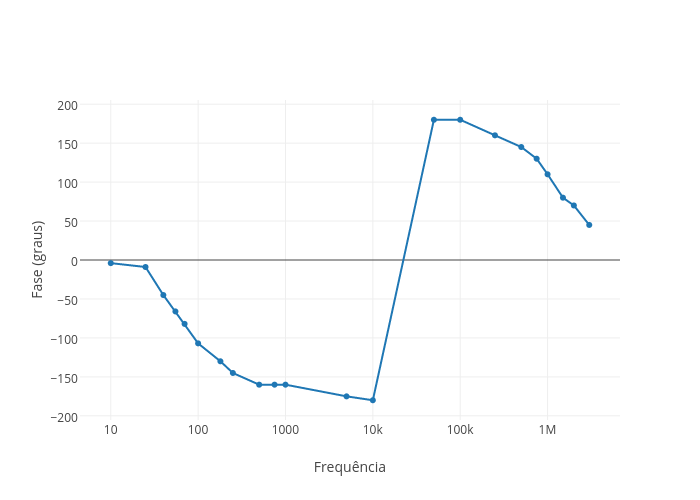
\includegraphics[width=0.8\linewidth]{img/RespFreq_ComReal_Fase.png}
\caption{Resposta em frequência com realimentação (Fase) }
\label{fig:resp_freq_com_real_fase}
\end{figure}


\subsection{Transformada Rápida de Fourier (FFT)}

\begin{figure}[H]
\centering
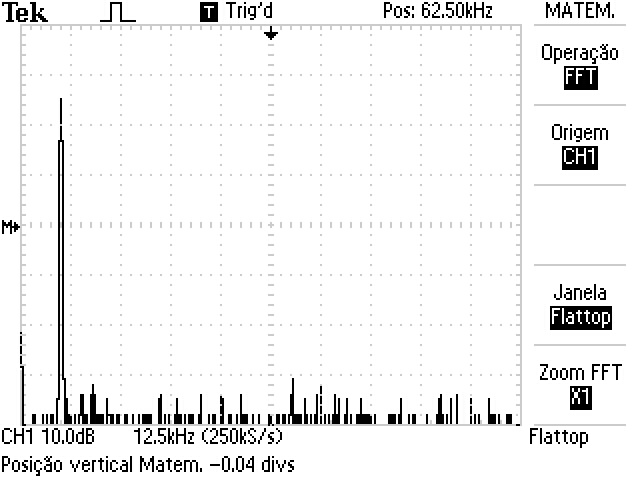
\includegraphics[width=0.8\linewidth]{img/FFT_ComReal.JPG}
\caption{FFT Com realimentação}
\label{fig:resp_freq_com_real_fase}
\end{figure}

\section{Amplificador classe B (Segundo experimento)}

\begin{table}[H]
\centering
\caption{Chave na posição 2}
\label{tab:ex2_pos2}
\begin{tabular}{|l|l|l|}
\hline
	Resistência & Av &  ganho\\ \hline
   	$0\omega$ & 5.2 & ganho mínimo \\ \hline
    $500k\omega$ & 383 & ganho máximo \\ \hline
\end{tabular}
\end{table}

\begin{table}[H]
\centering
\caption{Chave na posição 1}
\label{tab:ex2_pos2}
\begin{tabular}{|l|l|l|}
\hline
	Resistência & Av &  ganho\\ \hline
    $0\omega$ & 540 & ganho máximo \\ \hline
    $500k\omega$ & 4 & ganho mínimo \\ \hline
\end{tabular}
\end{table}

\begin{figure}[H]
\centering
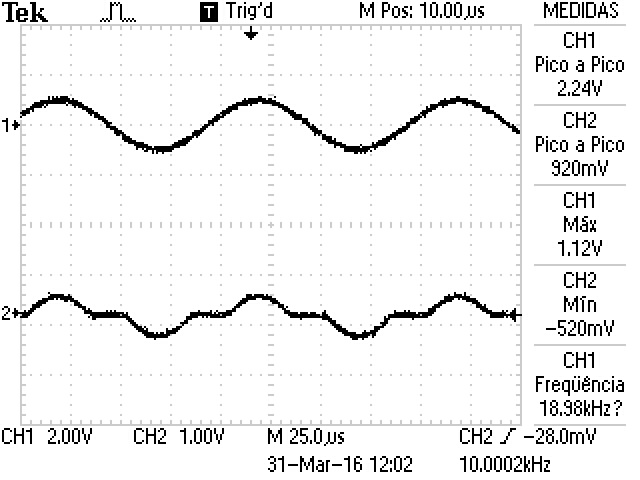
\includegraphics[width=0.8\linewidth]{img/Circ2_Distorcao1.JPG}
\caption{Distorção no ponto 2 com muita realimentação}
\label{fig:resp_freq_com_real_fase}
\end{figure}

\begin{figure}[H]
\centering
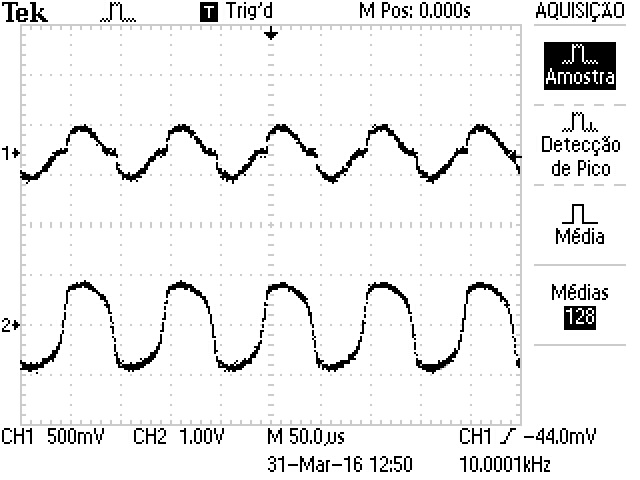
\includegraphics[width=0.8\linewidth]{img/Circ2_Distorcao2.JPG}
\caption{Distorção sendo jogada na entrada pela realimentação }
\label{fig:resp_freq_com_real_fase}
\end{figure}

\begin{figure}[H]
\centering
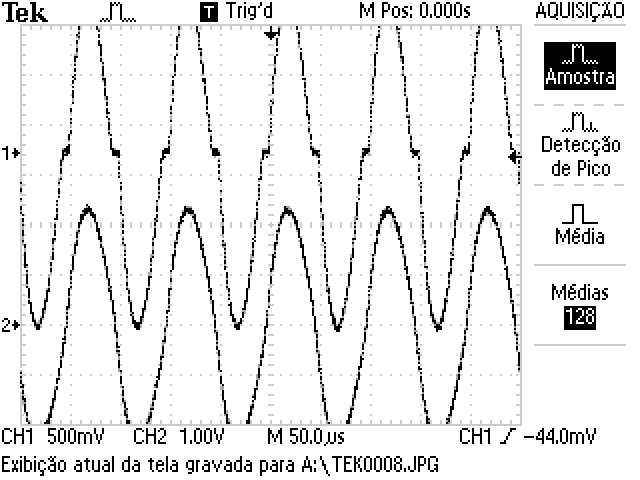
\includegraphics[width=0.8\linewidth]{img/Circ2_distorcao3.JPG}
\caption{Saída do circuito sem distorções}
\label{fig:resp_freq_com_real_fase}
\end{figure}

\chapter{Conclus\~ao}

Conclui-se com estes experimentos que a realimentação negativa melhora os parâmetros dos circuitos amplificadores, melhorando o controle de ganho, a impedância de entrada e de saída e a banda de resposta. Com ela também é possível melhorar a reasposta de resposta de circuitos com distorção (como amplificadores classes B), eliminando boa parte desta distorção. 

Entretanto, deve ser tomado alguns cuidados: a relimentação adiciona ao circuito uma pequena perda proveniente do efeito de carga, ela também só é aproveitável quando o ganho realimentado desejado é [muito] menor que o ganho do circuito sem realimentação. 

Mas talvez a característica que se deva tomar mais cuidado é com o risco do amplificador entrar em instabilidade devido ao deslocamento da fase para uma região inversora. Devido a isto, deve ser feito uma análise do diagrama de fase do diagrama do amplificador  para garantir que ele irá operar em uma região em que não ocorra instabilidade (fase se desloque 180º da fase de trabalho).

\bibliography{reflatex} % geracao automatica das referencias a partir do arquivo reflatex.bib

% --------- Lista de siglas --------
%\textbf{* Observa\c{c}\~oes:} a lista de siglas nao realiza a ordenacao das siglas em ordem alfabetica
% Em breve isso sera implementado, enquanto isso:
%\textbf{Sugest\~ao:} crie outro arquivo .tex para siglas e utilize o comando \sigla{sigla}{descri\c{c}\~ao}.
%Para incluir este arquivo no final do arquivo, utilize o comando \input{arquivo.tex}.
%Assim, Todas as siglas serao geradas na ultima pagina. Entao, devera excluir a ultima pagina da versao final do arquivo
% PDF do seu documento.


%-------- Citacoes ---------
% - Utilize o comando \citeonline{...} para citacoes com o seguinte formato: Autor et al. (2011).
% Este tipo de formato eh utilizado no comeco do paragrafo. P.ex.: \citeonline{autor2011}

% - Utilize o comando \cite{...} para citacoeses no meio ou final do paragrafo. P.ex.: \cite{autor2011}



%-------- Titulos com nomes cientificos (titulo, capitulos e secoes) ----------
% Regra para escrita de nomes cientificos:
% Os nomes devem ser escritos em italico, 
%a primeira letra do primeiro nome deve ser em maiusculo e o restante em minusculo (inclusive a primeira letra do segundo nome).
% VEJA os exemplos abaixo.
% 
% 1) voce nao quer que a secao fique com uppercase (caixa alta) automaticamente:
%\section[nouppercase]{\MakeUppercase{Estudo dos efeitos da radiacao ultravioleta C e TFD em celulas de} {\textit{Saccharomyces boulardii}}
%
% 2) por padrao os cases (maiusculas/minuscula) sao ajustados automaticamente, voce nao precisa usar makeuppercase e afins.
% \section{Introducao} % a introducao sera posta no texto como INTRODUCAO, automaticamente, como a norma indica.


\end{document}